% @author zhoulvwen
% zhou.lv.wen@gmail.com
\documentclass[12pt,a4paper,titlepage]{article}
\usepackage[left=1in,right=1in,top=1.5in,bottom=1.5in]{geometry}
\usepackage{amsthm, amsmath, amsfonts, amssymb, hyperref}
\usepackage{latexsym}
\usepackage{amssymb}
\usepackage{amstext}
\usepackage{fancyhdr}
\usepackage{mcode}
\usepackage{graphicx}
\usepackage[toc,page,title,titletoc,header]{appendix}
\usepackage{color}
\usepackage{titlesec}
\usepackage{lastpage}
\graphicspath{{figures/}}
\setlength{\parskip}{7.5pt plus 2pt minus 2pt}

\pagestyle{fancy} 
\lhead{Team \# 7380} 
\rhead{Page \thepage\ of \pageref{LastPage}} 

\setlength{\parindent}{0pt}
\begin{document}

\title{The Determination of the ``Sweet Spot" Base on Mechanics Simulation}
\author{\vspace{35pt}\\Zhou Lvwen\\Wang Fengge\\Yan Keqin\\ \vspace{35pt}}
\date{COMAP Mathematical Contest in Modeling\\February 22, 2010\\DaLian University, China}
\maketitle
%%%%%%%%%%%%%%%%%%%%%%%%%%%%%%%%%%%%%%%%%%%%%%%%%%%%%%%%%%%%%%%%%
\begin{abstract}
It is well known that there is a sweet spot on the bat, and it plays
an important role in baseball sport. In this paper, we address the
problem associated with three main portions include the position of
the sweet spot, the influences of the corked bat, and the
differences among different materials bat. We consider two important
models in hopes of solving the problems about the ``sweet spot".

The Plane Mechanics Model established by the \textbf{law of
conservation of momentum} is to solve the three main portions.
First, we analyze the direct impact of the ball and the bat, and
then get the relationship between the speed of the batted ball and
the hitting position, which makes sure the position of the sweet
spot where is not at the end of the bat. This model denies
``corking" a bat enhances the ``sweet spot" effect without
considering the corked bat easily controlled. Eventually, by using
the existing data about the different materials bat we know the
aluminum bat is better than the wood bat.

After presenting the above model, a \textbf{three-dimensional
Computer Model} which can \textbf{randomly simulate} the process of
athletes hit the ball in the ball park. From the simulation result,
We get the range of batted ball and find the standard deviation of
the range using the unmodified bat is larger than using the corded
bat, this is why the corked bat prohibited. On the other hand, it
explains the reason why the aluminum bat is prohibited by Major
League Baseball is that using a aluminum bat is contrary to the
principle of athletic, fairness and safety in the baseball games.

In conclusion, our algorithm is quite easy to implement and to solve
the problem successfully. Though there remain some weaknesses in our
model, it still has the significance for promoting to extensive use.
\end{abstract}


\newpage\tableofcontents\newpage

\section{Introduction}

With the popularity of the baseball, more and more people like the baseball sport. It is well-known to every hitter that there is a point which is called ``sweet spot" on the fat part of a baseball bat where maximum power is transferred to the ball when hit. And some players believe that ``corking" a bat (hollowing out a cylinder in the head of the bat and filling it with cork or rubber, then replacing a wood cap) enhances the ``sweet spot" effect. And more than that, the different materials bat will also affect the distribution of the sweet spot on the bat.

\subsection{Problem  Background}

On June 3, 2003, Chicago Cubs centerfielder Sammy Sosa was ejected from a game in the first inning for using a corked bat. His bat shattered upon impact with the ball and the umpire who picked it up discovered the bat had been hollowed out and filled with cork. Sammy said it was an accident that he had used the bat during batting practice and accidentally grabbed it by mistake when he went to the plate. Regardless of how the bat got there, it was not the first time a player has been caught with a doctored bat, and it won't be the last. But why not one raises the question ``Does the corked bat really enhance the effect of the `sweet spot'?" Is there any advantage (backed up by science) to using a corked bat?

Perceiving the sweet spot have conducted experiments directed at the question of whether one can perceive the sweet spot of a striking implement simply on the basis of wielding the implement and not just at the time of contact\cite{sweetspot}.

Trey Crisco et. al.\cite{DynamicPerformance} give a simulation only requires replicating the bat motion during the instant of contact with the ball, however invovles pure rotation.
Over the years, papers in this journal have addressed both experimental and theoretical issues associated with the baseball-bat collision. Bynamic FO et. al.\cite{PersonalCommunication} proves that the moden alumunim ans composite bats may hit a ball an average of 1 m/s(4 mph) faster than a traditional wooden bat.

\subsection{The explanation of the sweet spot}

Trying to locate the exact sweet spot on a baseball bat is not as simple a task as it might seem, because there are a multitude of definitions of the sweet spot. At present, there are seven different definitions about the sweet spot as followed:\cite{hollowsoftball}

\begin{itemize}
\item The location which produces least vibrational sensation (sting) in the batter's hands.

\item The location which produces maximum batted ball speed.

\item The location where maximum energy is transferred to the ball.

\item The location where coefficient of restitution is maximum.

\item The center of percussion.

\item The node of the fundamental vibrational mode.

\item The region between nodes of the first two vibrational modes.

\item The region between center of percussion and node of first vibrational mode.

\end{itemize}


From a player's viewpoint, the sweet spot is the place on the bat barrel where the contact between the bat and the baseball results in the best hit, the ball with the greatest speed when leaves the bat and his hands feel very little even no vibration from the impact. By looking up in lots of reference sources, we find there are two most frequent points of view about ``sweet spot", one regards it as the center of percussion (COP), which is the place on a bat or racket where it may be struck without a causing reaction at the point of support \cite{Percussion}, and the other is that it is the spot where the baseball gets the maximum instantaneous velocity when shot out of \cite{hollowsoftball}. In order to make it clear that what is the ``sweet spot", the first aspect that we should not only take into major consideration the speed of the ball gets, but also obtain some important findings through researching to make it apparent to the comfortable standard of the player.



\section{Problem Setup}

In this paper, we approach the problem in three main portions:

\begin{itemize}

\item The position of the sweet spot on the bat.

\item The impact on the sweet spot of the corked bat produces.

\item The differences the different materials bat make.
\end{itemize}

First, we create a plane mechanics model to solve the three portions. Next we establish a computer model to solve the three portions better. What's more, we have evaluated the influence of the sweet spot makes, and also solved why the corked bat and the aluminum bat are prohibited.

\section{Model 1: Plane Mechanics Model}

\subsection{The center of percussion}

In this part, we think that the center of percussion is the point on an object where a perpendicular impact will produce translational and rotational forces which perfectly cancel each other out at some given pivot point, so that the pivot will not be moving momentarily after the impulse. In addition, we study the reference of the Harvard University \cite{Percussion} seriously to find that we can obtain that the sweet spot is not at the end of the bat through proving the center of percussion is not in the top of bat. In the following article we will prove the center of percussion is not at the end of the bat.

Because the application time that the baseball acts on the bat is momentary, for the purpose of simplifying our model, we use the instantaneous impluse to solve the following problem. The moment when the ball hits the bat, its horizontal speed is far greater than the speed of the vertical direction, as a result, we could neglect its vertical speed in our model.

\begin{figure}[!htb]
\centering
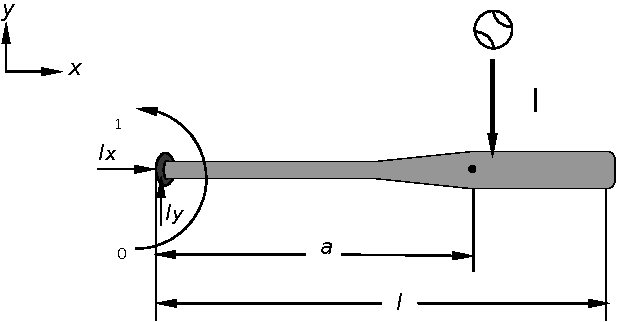
\includegraphics[width=0.6\textwidth]{batball.pdf}
\caption{\label{CollisionOfBaseballAndBat}collision of baseball and bat}
\end{figure}

By means of doing force analysis to the bat, the equations about the horizontal direction by the theorem of momentum and the momentum theorem of the vertical direction are

\begin{equation}
I_y-I=ma\omega_0-ma\omega_1, I_x=0
\end{equation}

Where
$I_y$ is the impulse that the bat to the athlete's hands in the horizontal direction,
  $I$ is the impulse that the ball to the bat,
  $a$ is the distance between the hand grip and the center of mass,
  $\omega_0$ is the bat's instantaneous angular velocity before collision,
  $\omega_1$ is the bat's instantaneous angular velocity after collision,
  $I_x$ is the impulse that the bat to the athlete's hands in the vertical direction.

In rapid sequence, we do the force analysis to the spot of the bat hand grip, and via the theorem of moment of momentum to obtain the following equation

\begin{equation}
-Ih=J\omega_0-J\omega_1
\end{equation}

Where $h$ is the distance between the hand grip and the center of percussion,
   $J$ is the moment of inertia of the bat.

As we all know that the center of percussion is the spot where the athlete's feelings are more comfortable, which means the athletes' hands are born the smallest impulse from the baseball bat, so that we can get the equation as followed

\begin{equation}
I_y=0
\end{equation}

Therefore, combine the equation 1,2,3, we have the 4th equation that is

\begin{equation}
h=\frac{J}{ma}
\end{equation}

In the following article, we will prove that $h$  is less than $l$ , meanwhile, according to the definition of moment of inertia, we can simply get the moment of inertia of the bat which is

\begin{equation}
J=\int_0^lx^2s(x)\rho\textrm{d}x
\end{equation}

Putting the above equation into the equation (4), we obtain

\[
\frac{h}{l}=\frac{\int_0^lx^2s(x)\rho\textrm{d}x}{\int_0^llxs(x)\rho\textrm{d}x}<1
\]


\textbf{Results Analysis}

By establishing and solving the above model ,we can obtain a result that $h<l$, which proves that the center of percussion is not at the end of the baseball bat, which is to say the sweet spot is not at the end of the bat. By analysising the results seriously, we find that the results match the general assumptions in our model, and what's more the results also match our expectations. Namely, it is worth pointing out are the facts that this method is in the ideal conditions (without making the errors by the player) to be raised. But in the actual baseball game, we have to take many factors into consideration, such as the weather, the competition area, the paychological factor of the athletes and so on. Besides, this method also makes the process of the hitting between the bat and the baseball ideal. This may be existent some difference when compared with the practical situation. However, as a consequence of these simplified in the real world are allowed, so we get the results of which also has a high credibility.


\subsection{The point which produces maximum batted ball speed}

Supposing the ball is being hit with the bat by direct impact, so we can know the baseball and the bat are always in the same plane of movement, Figure \ref{Motion} is a bat's trajectory\cite{EvaluatePredict}.

\begin{figure}[!htb]
\centering
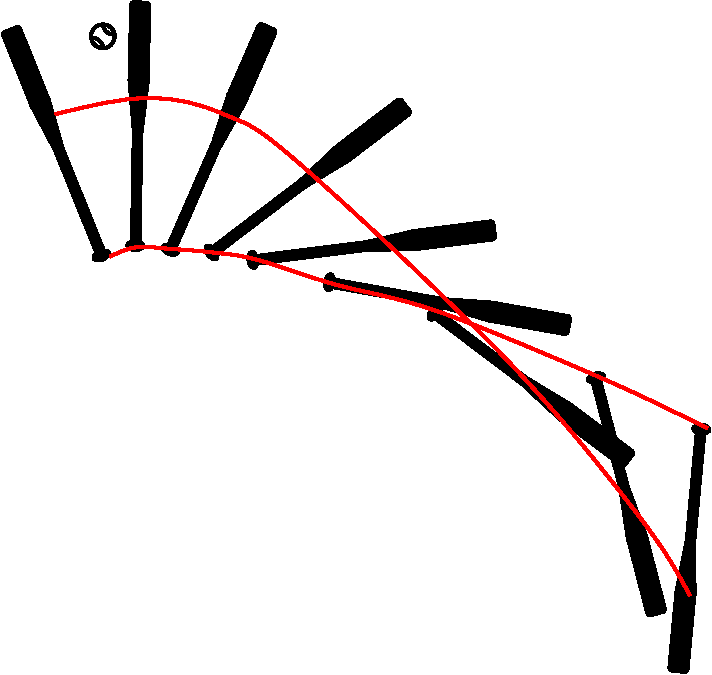
\includegraphics[width=0.6\textwidth]{motion.pdf}
\caption{\label{Motion}Motion of the swinging bat}
\end{figure}

Watts and Bahill also show that this rotational kinetic energy can be further broken down into a combination of two rotational motions, which can be used to derive an equation for batted-ball velocity. By analyzing the movement of the bat in figure \ref{Motion}, we can put its process of the motion broadly divided into two aspects of translational and rotational, as the Figure \ref{Varibales} shows. Ultimately, the process of these motions can be used to locate the bat to provide maximum energy transfer point, in other words, that is the sweet spot which the baseball can obtain the greatest speed.

\begin{figure}[!htb]
\centering
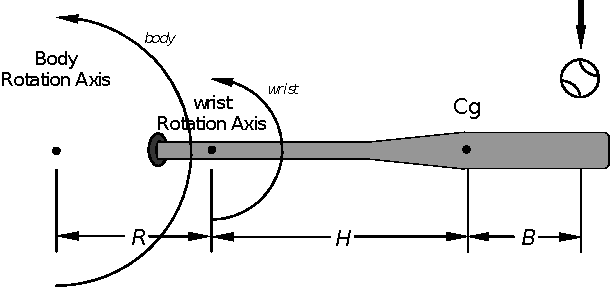
\includegraphics[width=0.6\textwidth]{basebat.pdf}
\caption{\label{Varibales}Variables denoted in swing equations}
\end{figure}


On the assumption that a batter's swing can be drawn as shown in Figure 3 where two angular velocity are applied to the bat: $\omega_{body}$ due to the rotation of the body and $\omega_{wrist}$ due to the rotation of the batter's wrists during the swing. The linear velocity of the bat at the $c_g (v_{2b})$ and at the point of impact ($v_B$) before a collision with the ball are

\[
v_{2b}=(R+H)\omega_{body}+H\omega_{wrist}
\]

\[
v_B=(R+H+B)\omega_{body}+(H+B)\omega_{wrist}
\]

Combining these two equations yields

\[
v_B=B(\omega_{body}+\omega_{wrist})+v_{2b}
\]

Making the substitution of $\omega_2 = \omega_{body} + \omega_{wrist}$ simplifies the equation further. And it is well known to us all that the total momentum for the bat and ball before and after the collision is conserved:

\begin{equation}
m_1v_{1b}+m_2(v_{2b}+\omega_{2b}B)=m_1v_{1a}+m_2(v_{2a}+\omega_{2a}B)
\end{equation}

Where $m_1$ is the mass of the ball, $m_2$ is the mass of the bat, $v_{1b}$ and $v_{1a}$ are the speed of the ball before and after collision, and $v_{b2}$ and $v_{a2}$ is the speed of the bat before and after collision.


During the bat-ball collision, we could suppose that the force exerted on the bat from the impact with the ball is $-F_1$, resulting in a torque on the bat about its $Cg$ is equal to $-BF_1$. Equating this torque over time $t$ to the change in angular momentum yields for the bat

\[
-BF_1t=I_0(\omega_{2a}-\omega_{2b})
\]

Similarly for the ball

\[
BF_1t=Bm_1(v_{1a}-v_{1b})
\]

Assuming that the rotational kinetic energy of the ball is negligible when compared to the translational kinetic energy. Conserving angular momentum between the bat and the ball during the collision produces

\begin{equation}
I_0(\omega_{2a}-\omega_{2b})+Bm_1(v_{1a}-v_{1b})=0
\end{equation}

The coefficient of restitution (COR) is defined as

\begin{equation}
e=\frac{v_{separate}}{v_{encounter}}=\frac{v_{1a}-v_{2a}-B\omega_{2a}}{v_{1b}-v_{2b}-B\omega_{2b}}
\end{equation}

where the COR is the negative ratio of the relative velocities of two bodies after and before a collision. The COR is not a value that is regarded as a material property because it not only depends on the material of both impacted bodies, but for nonlinear material systems, it also depends on the velocity at which they collide. It will also vary with respect to 9 different sizes, shapes and the temperature of the impacting bodies. For values of $e=1$, the collision is considered to be a perfectly elastic impact, that is, there is no energy loss due to the deformation of the bodies at impact. For values of $e=0$, the collision is considered to be a perfectly plastic impact. The relative velocity of the two bodies after impact is zero and the two particles move together at the same speed.

By integrating the above equations and using the Matlab software to solve, we get the baseball is shot out of a maximum speed of $v_{1a}$ (please see the annex to the \textbf{BatBallCollision.m} to get the process of the solution in detail).

\textbf{Results Analysis}


Through the solution process of the maximum speed $v_{1a}$ , we can get the result that the position of the sweet spot is not at the end of the bat. This result shows that our original conclusion concerning the position of the sweet spot is not at the end of the bat is quite correct, and it also proves that the empirical finding is wrong.

\subsection{The effect of the sweet spot of the corked bat}

The following arguments extracted from a reading of Robert Adair's book \textit{The Physics of Baseball}\cite{SwingWeights}

\begin{itemize}
\item \textbf{A corked bat has (slightly) less mass.} Because wood has been removed from the bat and replaced by some substances with a smaller density than wood, the bat is lighter by 1 to 2oz, depending on the dimensions of the cavity and the density of the filling substances. A bat which has less mass, and especially when it has a lower moment of inertia, may be swung faster. Potentially, 1.5oz does not much for an amateur player, but for a professional it means being able to watch the ball travel an additional 5 to 6 feet before having to commit to a swing.

\item \textbf{A corked bat's center of gravity closer to the hands.}Not only is the bat lighter, but the center of gravity and the balance point of the bat move closer to the hands. This means that the ''swing weight" of the bat is also reduced.

\item \textbf{A corked bat has lower inertia.} The moment of inertia (MOI) of the bat about the knob is reduced for a corked bat. You can think of the MOI as the ``rotational inertia" of the bat. Just like the ``inertia" or mass of an object measures the resistance of the object to a change in its translational motion, the rotational inertia measures the resistance to a change in its rotational motion. The effect is easy to understand: it is much easier to swing something when the weight is concentrated closer to your hands (smaller MOI) than when it is concentrated far from your hands (larger MOI).

\item \textbf{A corked bat means a less effective collision.} For a given bat speed, a heavier bat will produce a higher hit ball speed than a lighter bat. That is why the head of a golf driver is heavier than that of an iron: you want to drive the ball further. By reducing the weight at the barrel end of the bat, the efficiency of the bat is reduced, giving rise to a reduced hit ball speed and less distance on a long fly ball. This is the downside of using a corked bat.

\item \textbf{A corked bat has lower ball-bat COR (BBCOR).} Figure \ref{COR} shows a typical result for one of the bats. The plot indicates that the BBCOR is lowest for the drilled (hollow) bat. The BBCOR value for the corked bat is slightly lower than the original bat, though given the error in the measurements the results are basically indistinguishable. This result confirms the previous experiment by Alan Nathan that a corked bat does not have a trampoline effect.

\item \textbf{A corked bat could help the players make better ball control.} Because the bat is lighter and can be swung faster, a player can wait a few milliseconds longer before committing to a swing. This means he can watch the pitched ball travel about 5 to 6 or more feet before deciding to swing. For a junior player this may help make contact with the ball more often. But in other words, a corked bat will not make the ball go faster or further. Though we do not take into consideration this aspect in the Plane Mechanics model immediately, we will consider it in our following computer model.

\end{itemize}

\begin{figure}[!htb]
\centering
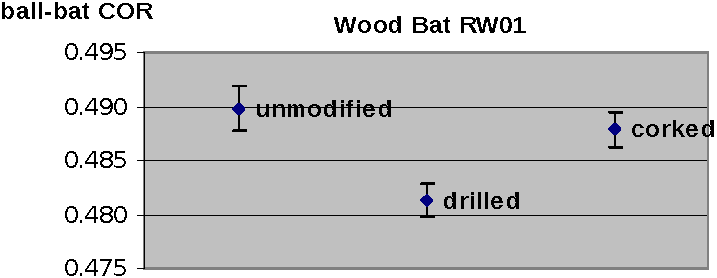
\includegraphics[width=0.8\textwidth]{batcor.pdf}
\caption{\label{COR}Measured values of the ball-bat coefficient of restitution (COR) for an unmodified, drilled, and corked wood bat, as explained in the text. The error flags indicate the standard deviation of the mean of the measurements. These data demonstrate that there is no measureable trampoline effect when a wood bat is drilled or corked.\cite{RemarksCorked}}
\end{figure}

According to the above description of the data for a corked bat, and making reference to a number of unmodified baseball bat data, we can make reasonable assumptions about the two kinds of the bat in the following analysis, as shown in the table \ref{parametersCorked}.

\begin{table}[!htb]
\centering
\caption{\label{parametersCorked}The parameters of Unmodified and Corked That we assumed}
\begin{tabular}{|l|l|l|l|l|l|}
\hline
\multicolumn{1}{|c|}{Baseball } & \multicolumn{1}{c|}{Length} & \multicolumn{1}{c|}{Weight} & \multicolumn{1}{c|}{Bp} & \multicolumn{1}{c|}{MoI6} & \multicolumn{1}{c|}{e} \\
\multicolumn{1}{|c|}{Bat} & \multicolumn{1}{c|}{($in$)} & \multicolumn{1}{c|}{($oz$)} & \multicolumn{1}{c|}{($in$)} & \multicolumn{1}{c|}{($oz-in^2$)} & \multicolumn{1}{c|}{} \\
\hline
\multicolumn{1}{|c|}{Unmodified} & \multicolumn{1}{c|}{34} & \multicolumn{1}{c|}{35} & \multicolumn{1}{c|}{22} & \multicolumn{1}{c|}{11000} & \multicolumn{1}{c|}{0.490} \\
\hline
\multicolumn{1}{|c|}{Corked} & \multicolumn{1}{c|}{34} & \multicolumn{1}{c|}{33} & \multicolumn{1}{c|}{20} & \multicolumn{1}{c|}{8000} & \multicolumn{1}{c|}{0.482} \\
\hline
\end{tabular}
\end{table}

Taking the data of table \ref{parametersCorked} into the MatLab program to get the relationship between the speed of the ball and the distance which is from the hit point to the end of the bat, and it will be shown in the figure \ref{VelocityDistance}.

\begin{figure}[!htb]
\centering
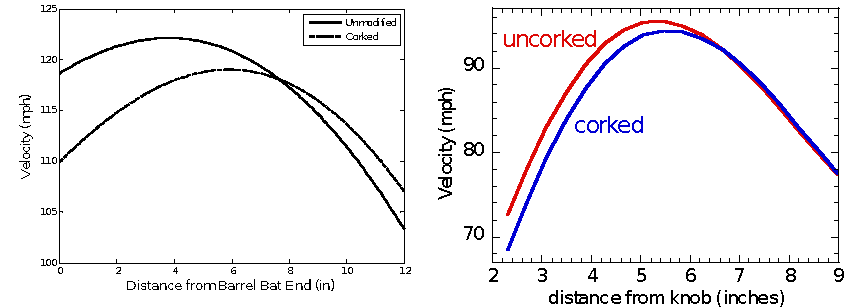
\includegraphics[width=1\textwidth]{distance.pdf}
\caption{\label{VelocityDistance}Velocity vs. Distance between collision point and Barrel Bat end.  The left figure which is we create in the model to obtain, and the right figure is extracted from the reference \cite{RemarksCorked}. By observing the analysis, we find that the results obtained in our model is are very similar with the literature. Therefore, the fact shows that to some extent our model is reasonable.}
\end{figure}


\textbf{Results Analysis}

We can see that in the the figure 5, both the results in the literature and the results of our paper could be seen that a corked bat will not play longer than the uncorked bat. By this model, we can deny that the cocked bat performs better than the traditional bat.

\begin{itemize}
\item The maximal velocity of the uncorked bat is slight bigger than the cocked bat.

\item The sweet spot of the uncorked bat is more close to the end of the bat than the corked bat.

\item The sweet spot zone of the uncorked bat is wider than the corked bat.
\end{itemize}

We conclude that the main reason may be that we do not consider the ball control factor, and we also think the reference did also not take the factor into consideration. However, we will take it into account in the following computer model, and make a further explanation that the effect which the corked bat makes.

\subsection{The differences between the wood and aluminum bats }

It is known to all that the physical differences between wood and metal baseball bats are quite obvious. But if both of them have the same mass, their structure will be very different, the metal bat must be hollow. In this part, we think the effect of the aluminum is better than the wood bat when use them to hit the baseball.

Usually, a solid wood bat weighs 2 units less than its length, on the other hand, a hollow metal bat weighs either 3 or more units less than its length. In addition to the above different factors between wood and metal baseball bats, a significant difference between wood and metal bats is the energy-transfer mechanism between the bat and the baseball during the collision.

However, the difference between the energy-transfer mechanisms is a fundamental result of the wood bat being solid and the metal bat being hollow.That is to say that we can create a model to predict the different behavior about wood(usually ash) or metal(usually aluminum) bats.

In our model, we also use the wood and aluminum bat to solve the problem. There is some information with regard to the two different types of the bats as shown in the table and figure \ref{correspondingparameters}\cite{hollowsoftball}.

\begin{figure}[!htb]
\centering
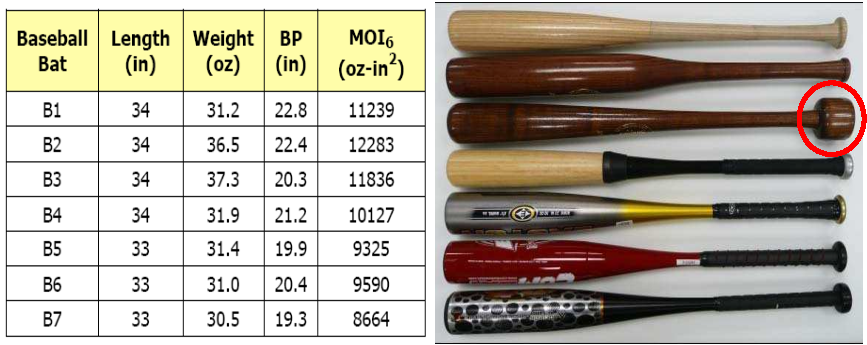
\includegraphics[width=0.8\textwidth]{figtab.pdf}
\caption{\label{correspondingparameters}Different bats and their corresponding parameters\cite{Swing_Weights}}
\end{figure}


We can demonstrably know the weight, balance point and moment of inertia about 6-in point on the hand grip on the bat by a sampling of 34-inch wood baseball and 33-inch aluminum or composite bats comparing combinations in the figure \ref{correspondingparameters}(left). Simultaneously, we give a figure whose different bats via descending order from top to bottom are one-to-one correspondence with the parameters in the figure \ref{correspondingparameters}(left). Quite obviously, we find that the third bat is different from the other bats in the figure \ref{correspondingparameters}(right), and we have already come out it with a red circle. We caculate this will make some different results in our following plot. \cite{hollowsoftball}

In addition, there are extra difference that we must take into account.

\begin{itemize}
\item \textbf{Aluminum bats can be swung faster.} Comparison of wood and aluminum bats, an aluminum bat with the same weight as a wood bat will have a significantly lower inertia and a player can swing a lower inertia bat faster.(we set aluminum bat velocity = 106.5 and wood = 98.6)

\item Aluminum bats have the ``trampoline effect". When a ball hits a wood bat, it compresses to nearly half its original diameter, losing up to 75\% of its initial energy to internal friction forces during this compression. In a hollow bat, however, the bat barrel compresses somewhat like a spring, when the ball impacts it.(we set aluminum bat COR = 0.5 and wood =0.45);
\end{itemize}

By substituting the different parameters of the baseball bats in the figure 6(left)into the $v_{1b}=F(B,L,m,BP,I)$ representative values for wood and metal bats, a plot of the batted-ball velocity as a function of the location of the impact point on the bat from the barrel end can be created.


\begin{figure}[!htb]
\centering
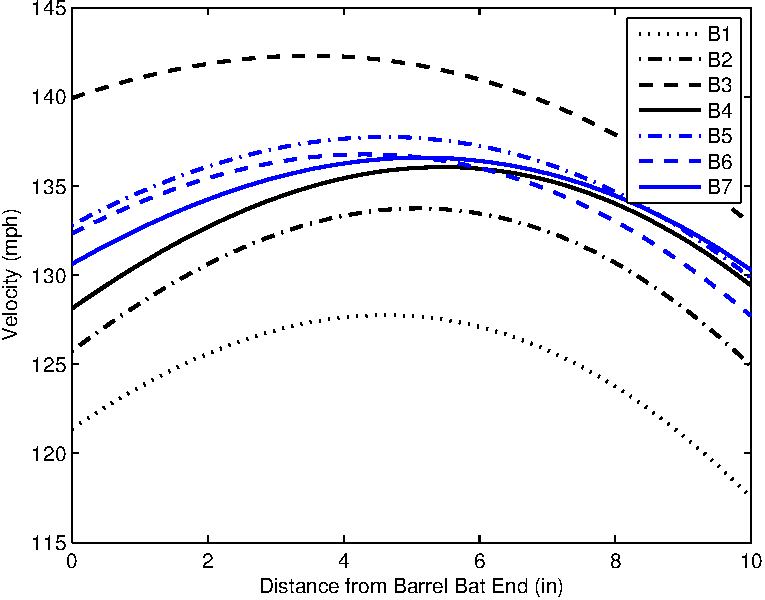
\includegraphics[width=0.6\textwidth]{fig01m1.pdf}
\caption{\label{Plotdemonstrating}Plot demonstrating Equation}
\end{figure}

In this figure, combining the maximum speed $v_{1b}=F(B,L,m,BP,I)$ we can obtain the functional relations between the maximum speed and the distance from striking point on the ball to the end of the bat. We can easily find that the place where the sweet spot on the bat is and the B3 curve is different from the other curves distinctly. Namely, we also find the metal bat is better than the wood bat when used to hit the baseball in the figure.

\textbf{Results Analysis}

From the above figure \ref{Plotdemonstrating}, we can come to the results that:

\begin{itemize}

\item \textbf{The peaks show where along the length of the bat the maximum energy transfer occurs.} We obtain the result the location of the maximum energy transfer is commonly referred to as the sweet spot on the bat, at the same time it proves the sweet spot is not at the end of the bat again and explains our previous model is correct and feasible again.

\item \textbf{Both the materials and the shape structure will have an effect on the ``sweet spot" effect.}
 We find that the B3 curve is different from the others, this responds our previous conclusion that its special structure makes it different, on the other hand, this explains that our model is feasible.

\item \textbf{The aluminum bat is better than the wood bat.} We analyze the differences between the wood and metal bat with the figure \ref{Plotdemonstrating}, and we get the result that the aluminum bat is better than the wood bat. This also explains the different materials have effects on batting. But on account of the aluminum bat can hit the baseball faster and farther, it makes the athletic competition reduce more, and it is also unfair to the competitors who use the wood bat. Therefore, for the purpose of the principle of athletic and fair play, the metal wood should be prohibited in the baseball game. Maybe it is the reason why Major League Baseball prohibits metal bats. However, for a beginner the metal bat is still a better tool to learn.

\end{itemize}

\section{Model 2: Computer Model}

In this Model,we will establish a three-dimensional Model
based on the model 1.

\begin{figure}[!htb]
\centering
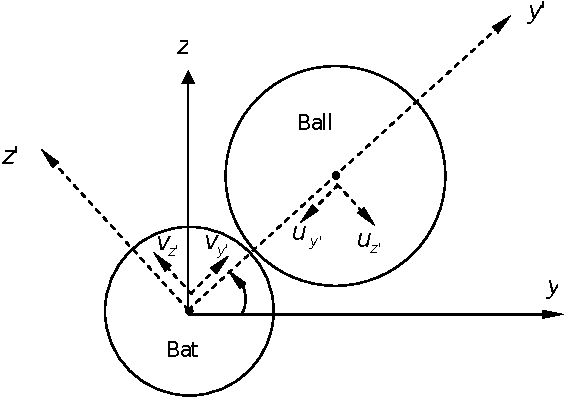
\includegraphics[width=0.6\textwidth]{computer.pdf}
\caption{\label{computermodel}Initial vertical configuration of the bat/ball collision. (Where $x$ and $x'$ axis perpendicular to the paper outwards, the figure is not drawn)}
\end{figure}


As the Figure \ref{computermodel} shows, the momentum of the $y'$  direction between the bat and ball before and after the collision is conserved:

\[
Mv'_{y0}+mu'_{y0}=Mv'_y+mu'_y
\]
On the assumption that the rotational kinetic energy of the ball is negligible when compared to the translational kinetic energy. Conserving angular momentum between the bat and the ball during the collision produces

\[
I_0(\omega-\omega')+Bm(u'_y-u_y)=0
\]

The COR is defined as

\[
e=\frac{u'_y-v'_y}{u'_{y0}-v'_{y0}}
\]

In fact��the above model concerning the velocity fluctuation of the  $y'$ direction is the previous simple model which is already established. But in the computer model, we do not take into consideration the friction effect of the instant of collision, so we have the following equations which are

\[
v'_z=v'_{z0}, u'_z=u'_{z0}
\]

\[
v'_x=v'_{x0}=0, u'_x=u'_{x0}
\]

In fact, the friction effect will make the velocity change in both the $x'$  direction and the $z'$ direction, and could also cause the rotational motion of the ball happens. However, we believe that ignoring the role of friction will not make our results have larger errors. And by doing this, we gain the result that the sweet spot is not at the end of the bat once again, it proves our model is correct and feasible.

We proceed from the simple model to establish a general three-dimensional model, and use the computer to go on with analog simulation. In each analog simulation of our model, we will make the following parameters be set to normally distributed random numbers, thus we can simulate the process of the batting, and this will be closer to the reality. Simultaneously, we can also use the process of the batting to respond the different levels about the players by the setting a random numbers, especially the typical value and the variance. As a result, when we set the random numbers preferable can it respond to people with a higher level of batting, conversely, it will reflects the player to be a beginner. The parameters as shown followed:

\begin{itemize}
\item The ball's initial velocity (including direction).

\item The bat's initial velocity (including direction).

\item The distance between the point of impact and the sweet spot determined by model 1.

\item The height from hitting position to the ground.

\item The $\theta$ angle in the figure \ref{computermodel}.
\end{itemize}

\subsection{The effect of the sweet spot of the corked bat}

To analyze the effects of the different types of the bats which are unmodified or corked when hit the baseball, we created different simulations batting by varying our parameters. We then ran each simulations batting strategy on these different parameters to get the hitting ranges for each bat, and our initial inference is that the corked bat will be better than the unmodified bat for the latter can not make the player control easier when hitting the baseball. In particular, our goal through these simulations is to determine which of the bats has the greatest effect of the sweet spot on the simulated performance of the different structures. As a result, we get the figures to explain whether the unmodified bat or the corked bat is better to be used, as shown in the Figure \ref{Fieldcorked}.

\begin{figure}[!htb]
\centering
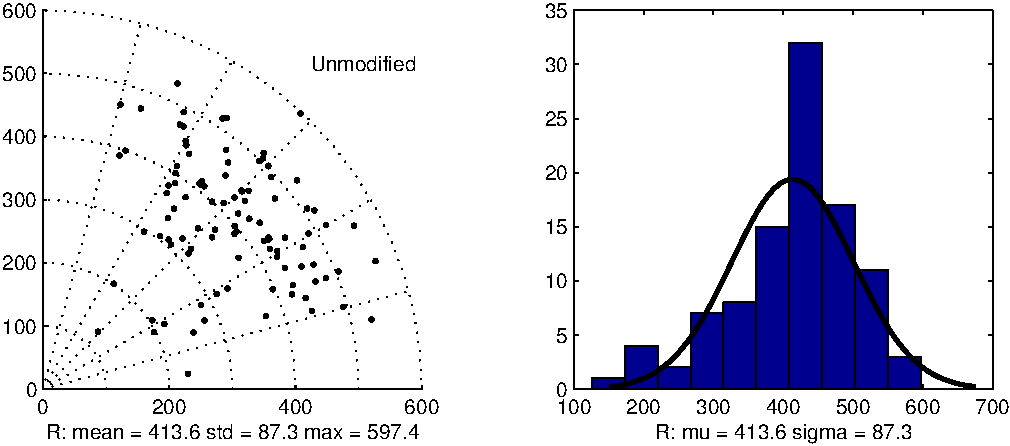
\includegraphics[width=0.71\textwidth]{unmodifiedm2.pdf}\\
.\\
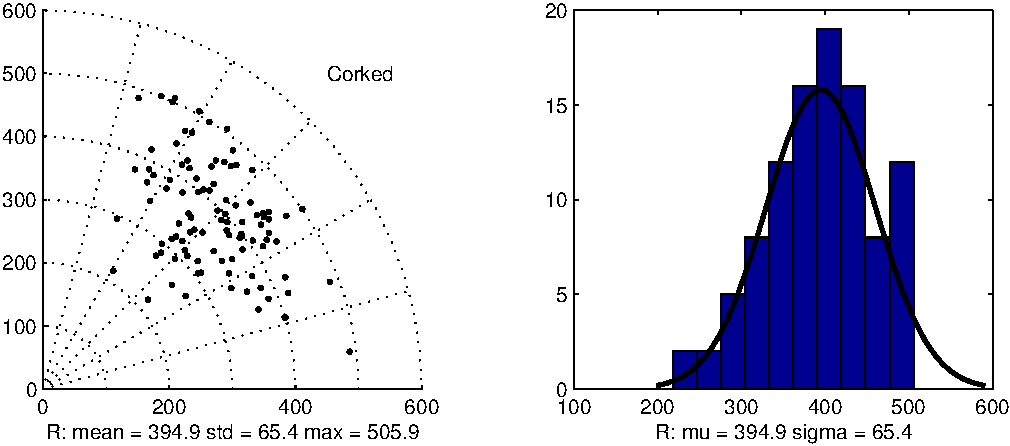
\includegraphics[width=0.71\textwidth]{corkedm2.pdf}\\
\caption{\label{Fieldcorked}Field locations of the corked bat bats baseballs and its range distribution. Both the above and the under figure on the left side represent respectively the field locations of batted baseballs, and both the above and the under figure on the right reflect respectively the distribution of the hitting range which is from (0,0) to the baseball's landing point.}
\end{figure}

Note: Because when using the corked bat to hit the baseball could make the player have a longer reaction time to control the motion of the baseball [see the above explanation in the Plane Mechanics Model] , the standard deviation about the ball hits the vicinage of the sweet spot (namely, the sweet spot zone) that we get by using the unmodified bat is larger than using the corked bat when we make simulation, that is to say that the probability of the baseball hits the sweet spot zone is much larger when using a corked bat. It confirms that ``corking" a bat could enhance the "sweet spot" effect. For this reason, the principle of the athletic and fair play can not be represented in the baseball game.

Although the speed of the baseball was shot out of reduces, on the other hand, as long as the second or the third rampart has enough time to be able to score, the corked bat is a better one. Therefore, a corked bat may be only used to make ball control to get scores better. However, the current problem is that no one knows whether it is real that a corked bat acts worse than the uncorked, so in lots of baseball games the corked bat are still not allowed to use. Maybe the corked bat is able to improve its breakage rate and reduce the difficulty of the game, so for the purpose of the principle of safe and fair play, the corked bat is prohibited.

\subsection{The differences between the wood and aluminum bats}

For good measure, with the view of explaining the different effects between the wood and metal bats, we have also taken into consideration some of the above parameters to talk about the differences between the wood and metal bats. Furthermore, by changing the different parameters, we produce the plots measuring the effectiveness of the various materials bat concerning the speed when the two types of the bats hit the baseball, field locations of the baseball's landing sites and the distributions of the baseball's hitting range and so on by conducting a computer simulation. In the following article, we will show the differences by means of the figure \ref{Fieldwood}.

\newpage

\begin{figure}[!htb]
\centering
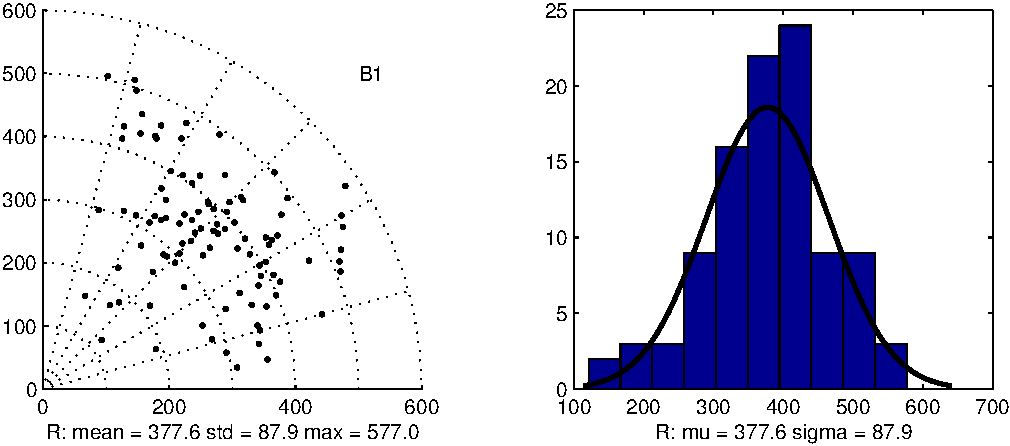
\includegraphics[width=0.71\textwidth]{b1.pdf}\\
.\\
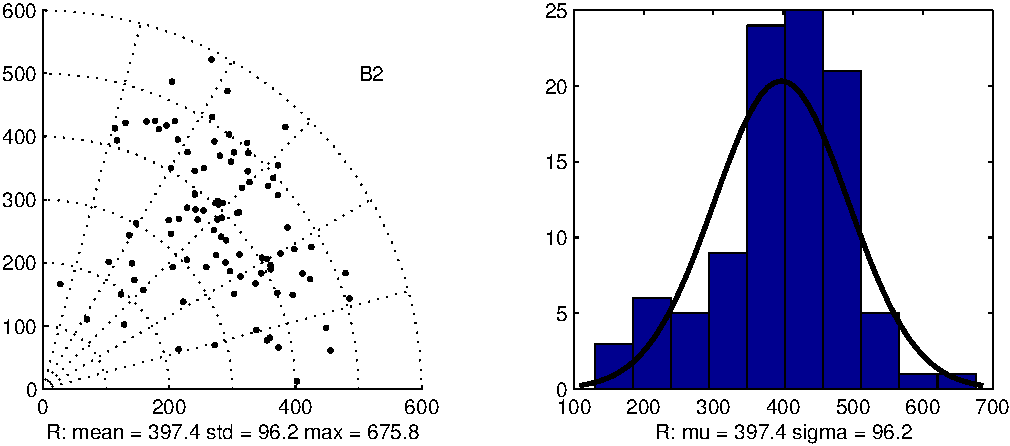
\includegraphics[width=0.71\textwidth]{b2.pdf}\\
.\\
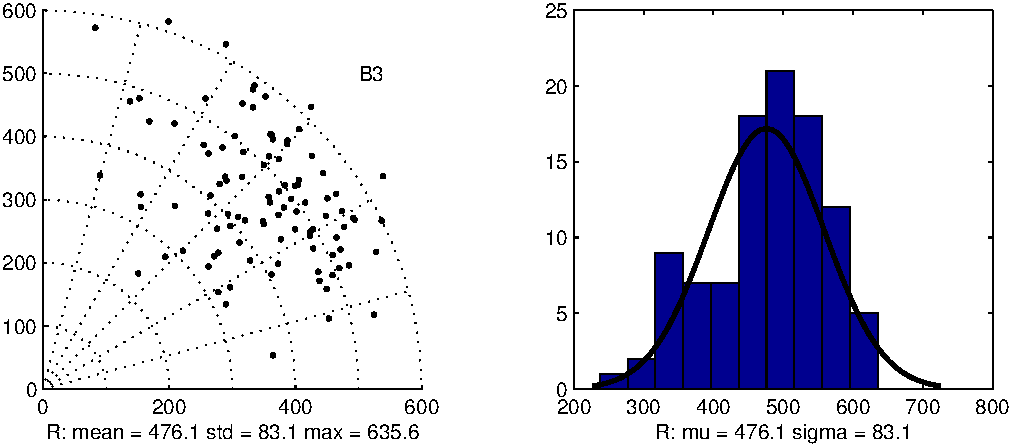
\includegraphics[width=0.71\textwidth]{b3.pdf}\\
.\\
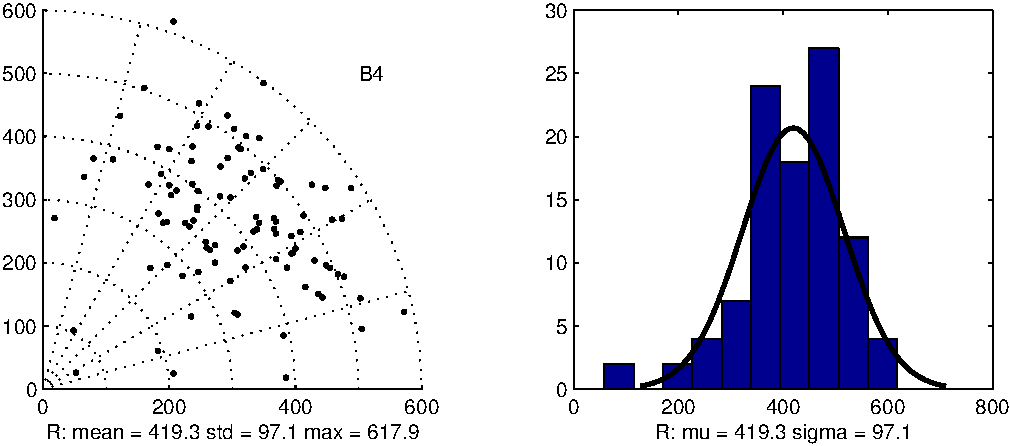
\includegraphics[width=0.71\textwidth]{b4.pdf}\\
\end{figure}

\begin{figure}[!htb]
\centering
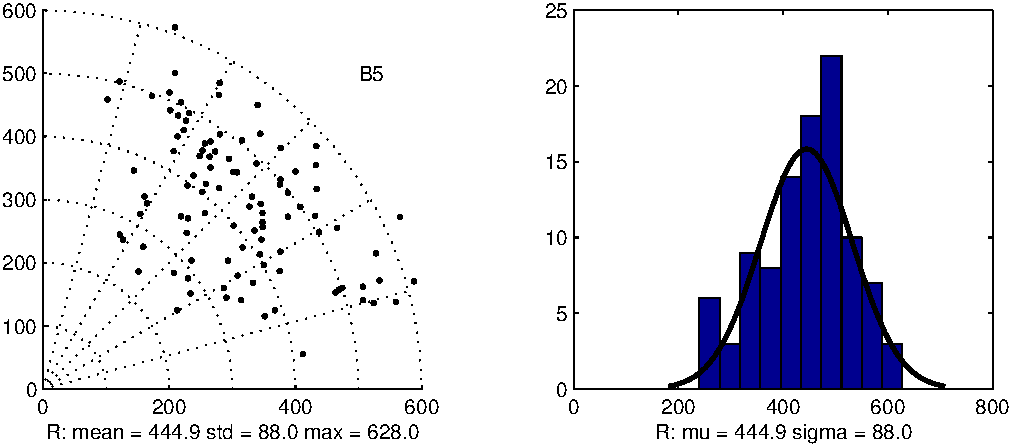
\includegraphics[width=0.71\textwidth]{b5.pdf}\\
.\\
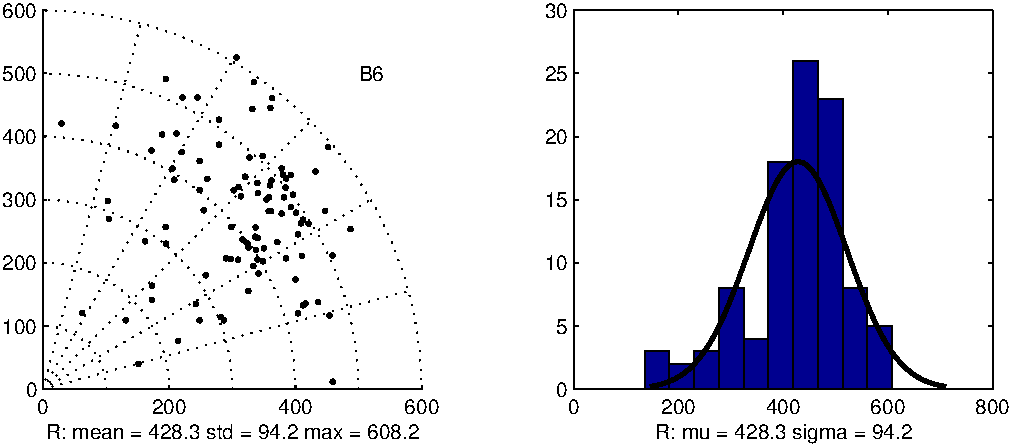
\includegraphics[width=0.71\textwidth]{b6.pdf}\\
.\\
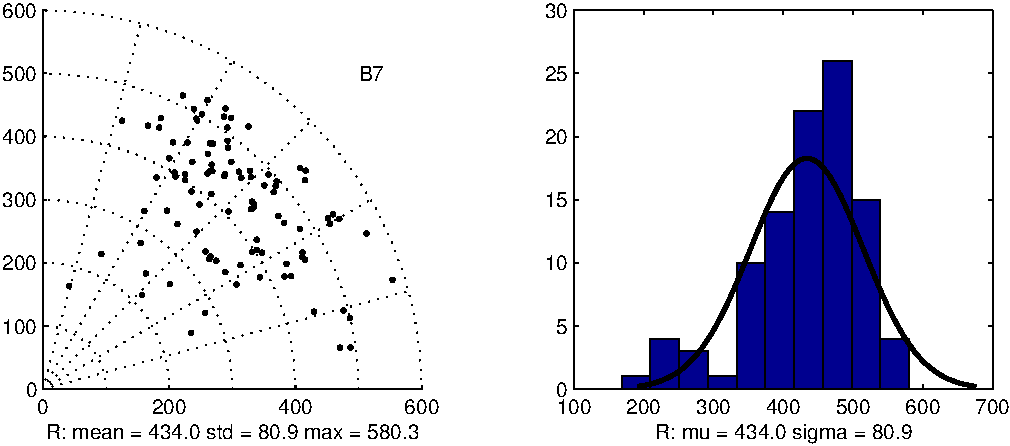
\includegraphics[width=0.71\textwidth]{b7.pdf}\\
\caption{\label{Fieldwood}Field locations of the wood(B1-B4) and metal(B5-B7) bats batted baseballs and their range distribution. Both the above and the under figure on the left side represent respectively the field locations of batted baseballs , and both the above and the under figure on the right reflect respectively the distribution of the hitting range which is from (0,0) to the baseball's landing point.}
\end{figure}

As everyone knows that in the same conditions, the aluminum bat hits the baseball with a longer distance than the wood bat does in general(bat B3 is performance different in evidence from the other wood bats, this responds our previous conclusion that its special structure makes it different, see model 1 and figure \ref{correspondingparameters}). From the figure we can see that the average velocity is 20 inches faster when hit by the aluminum than the wood bat, but the standard deviation between the two different kind of the bats is almost identical. However, in order to improve the competitive nature of the baseball games, in the rules of the baseball game the aluminum bat is prohibited to use.


\section{Results}

Here, comparing the results of each problem obtained in the Computer Model with those that got in the Plane Mechanics, we find that both the two results are surprisingly consistent, which explains that both the previous and the latter model we establish are feasible to some extent. In addition to that, in the Computer Model, we obtain the place of the sweet spot on the bat is not at the end of the bat, too.

Namely, it has also made more convincing evidence to explain whether the corked bat could enhance the ``sweet spot" effect. At the same time, it also better explains the reasons why Major League Baseball prohibit ``corking", which are that the corked bat could extend the reaction time for the batter to hit the baseball, and also let the batter make ball control better. But the level of this kind of the ball control is not able to reflect the athletes�� real competitive level, it is contrary to the principle of the baseball game��s athletic. Besides, the corked bat is easily broken and its safety is not better to use, this may be a reason why it is prohibita (In the USA, the human rights are quite important).

In rapid sequence, we find that the different materials bat have the different influences when hitting the baseball. The effect of the metal bat is better than the wood bat obviously, the most possible reason is that the aluminum bat is hollow when compared with the wood bat with the same mass. This easily makes the baseball obtain a greater speed, which let the competition easier to hit and much more unfair to those who use the wood bats. As a result, for the sake of improving the level of the athletic and fairness about the competition, we think this may be the main reason why Major League Baseball prohibits metal bats.

\section{Strengths and Weaknesses}

\subsection{Model 1}

\textbf{Strengths}

In the Model 1, we take into account the major factors of affecting the ``sweet spot" according to the Law of Conserving Momentum, Law of Conserving Angular Momentum and Coefficient of restitution. By doing this, we are able to obtain the mathematic relationship between the hitting spot and the batting speed, thereby track the so called ``sweet pot". This not only can interpret the ``sweet pot" is not at the end of the bat, but also allows our model to evaluate and compare the ``sweet spot" effect of different bats which based on different parameters.

The results not only are consistent with the conclusions of related references, but also accord with the computing model. Using this model, our approach allowed us to isolate the random factors and the three-dimensional space, so as to obtain the certain results according to the specific parameter.


\textbf{Weaknesses}

While our model attempted to model the ``sweet pot" effect of different bat based on different parameters accurately, it was of cause impossible to completely capture random factors, including the velocity of ball and bat before hitting and hitting spot. Further, we just only take into account the one-dimensional space (direct impact), which lead to inevitable restriction.

In addition, we only considered value of the velocity before hitting, while we did take into account the direction of the velocity, so that we can not calculate the shot distance of the ball. While using the computing model did allow us to improve upon the model 1, further improvements will be available by examining other possibilities.

\subsection{Model 2}

\textbf{Strengths}

In the model 2, we modify the model from one-dimensional to three-dimensional based on the model 1.That means we not only consider the direct impact, but also take into account skew impact, which is more consistent with actual hitting process. Further, we consider the random factors, including the velocity of ball and bat before hitting and hitting spot, which accord with the actual case.

In addition, by doing this, we not only can simulate the hitting process of different baseball player and different bat, but also we can calculate the shot distance and its distribution function. This model has solved the restrictions of model 1, which make further improvements available.

\textbf{Weaknesses}

While this model can consider the random factors of hitting process, we have ignore the friction between the ball and the bat, so as to consider that the ball cannot circumgyrate, which is not consistent with the actual process. However, the friction is so small compared with hitting impact and the hitting time is so extremely short that the friction has little impact on the results. Hence, the error is neglect able.

In addition, we ignore the effect of the air friction on the shot distance, which makes the results of shot distance bigger than the actual value. While in fact this will not affect the comparisons of ``sweet spot" effect between different bats based on different parameters.



\section{Alternative Approaches and Future Work}

There were several extensions to our model and simulation that we could not pursue due to the time constraint. We considered evaluating the ``sweet spot" effect of different bat by counting the probability of take the sack and the probability of home runs. We would then be able to compare advantages and disadvantages of different bat in practical baseball field. 

%%%%%%%%%%%%%%%%%%%%%%%%%%%%%%%%%%%%%%%%%%%%%%%%%%%%%%%%%%%%%%%%%
\newpage
\begin{thebibliography}{99}

\bibitem{sweetspot}Carello, C., Thuot, S., Andersen, K. L., \& Turvey, M. T. (1999). Perceiving the sweet spot. Perception, 28,1128-1141.
%1
\bibitem{DynamicPerformance}Bryant FO, Burkett LN, Chen SS, KrahenBuhl GS, Lu P. Dynamic and performance characteristics of baseball bats. Rec Q Exerc Sport 1979;48:505-10.
%2
\bibitem{PersonalCommunication}Trey Crisco, Personal communication, Brown University, 1999.
%3
\bibitem{hollowsoftball} Daniel A. Russell, ``The sweet spot of a hollow baseball or softball bat",\\http://paws.kettering.edu/~drussell/bats-new/sweetspot.html,February 19th, 2010.
%4
\bibitem{Percussion} ``Center of Percussion",\\
http://www.fas.harvard.edu/~scidemos/NewtonianMechanics/CenterofPercussion/CenterofPercussion.html,February 19th, 2010.
%5
\bibitem{EvaluatePredict} TIMOTHY J. MUSTONE, A Method to Evaluate and Predict the Performance of Baseball Bats Using Finite Elements. B.S.M.E. UNIVERSITY OF MASSACHUSETTS LOWELL (1996)
%6
\bibitem{SwingWeights} Dan Russell, Kettering University, "Swing Weights of Baseball
and Softball Bats", Submitted to The Physics Teacher, April 17,2009.
%7
\bibitem{Physics} Robert K. Adair, The Physics of Baseball, 3rd Ed., (Harper Collins, 2002)
%8
\bibitem{RemarksCorked} Some Remarks on Corked Bats \\
http://webusers.npl.illinois.edu/~a-nathan/pob/corked-bat-remarks.pdf
%9
\bibitem{Swing_Weights}  Dan Russell, Swing Weights of Baseball and Softball Bats.
%10
\end{thebibliography}

\newpage
\appendix
\appendixpage
\begin{subappendices}

\section{MatLab Script of Model 1}

\textbf{Main1model1.m}

\lstinputlisting{./matlab/model1/Main1model1.m}

\textbf{Main2model1.m}

\lstinputlisting{./matlab/model1/Main2model1.m}

\textbf{Main3model1.m}

\lstinputlisting{./matlab/model1/Main3model1.m}

\textbf{BatBallCollision.m}
\lstinputlisting{./matlab/model1/BatBallCollision.m}

\section{MatLab Script of Model 2}

\textbf{Main1model2.m}

\lstinputlisting{./matlab/model2/Main1model2.m}

\textbf{Main2model2.m}

\lstinputlisting{./matlab/model2/Main2model2.m}

\textbf{Main3model2.m}

\lstinputlisting{./matlab/model2/Main3model2.m}

\textbf{battest.m}

\lstinputlisting{./matlab/model2/battest.m}

\textbf{RotAxis.m}
\lstinputlisting{./matlab/model2/RotAxis.m}

\textbf{BatBallCollision.m}
\lstinputlisting{./matlab/model2/BatBallCollision.m}

\textbf{plotaxis.m}
\lstinputlisting{./matlab/model2/plotaxis.m}
\end{subappendices}

\end{document}

